\documentclass[hidelinks,12pt]{article}
\usepackage[left=0.25cm,top=1cm,right=0.25cm,bottom=1cm]{geometry}
%\usepackage[landscape]{geometry}
\textwidth = 20cm
\hoffset = -1cm
\usepackage[utf8]{inputenc}
\usepackage[spanish,es-tabla]{babel}
\usepackage[autostyle,spanish=mexican]{csquotes}
\usepackage[tbtags]{amsmath}
\usepackage{nccmath}
\usepackage{amsthm}
\usepackage{amssymb}
\usepackage{mathrsfs}
\usepackage{graphicx}
\usepackage{subfig}
\usepackage{standalone}
\usepackage[outdir=./Imagenes/]{epstopdf}
\usepackage{siunitx}
\usepackage{physics}
\usepackage{color}
\usepackage{float}
\usepackage{hyperref}
\usepackage{multicol}
%\usepackage{milista}
\usepackage{anyfontsize}
\usepackage{anysize}
%\usepackage{enumerate}
\usepackage[shortlabels]{enumitem}
\usepackage{capt-of}
\usepackage{bm}
\usepackage{relsize}
\usepackage{placeins}
\usepackage{empheq}
\usepackage{cancel}
\usepackage{wrapfig}
\usepackage[flushleft]{threeparttable}
\usepackage{makecell}
\usepackage{fancyhdr}
\usepackage{tikz}
\usepackage{bigints}
\usepackage{scalerel}
\usepackage{pgfplots}
\usepackage{pdflscape}
\pgfplotsset{compat=1.16}
\spanishdecimal{.}
\renewcommand{\baselinestretch}{1.5} 
\renewcommand\labelenumii{\theenumi.{\arabic{enumii}})}
\newcommand{\ptilde}[1]{\ensuremath{{#1}^{\prime}}}
\newcommand{\stilde}[1]{\ensuremath{{#1}^{\prime \prime}}}
\newcommand{\ttilde}[1]{\ensuremath{{#1}^{\prime \prime \prime}}}
\newcommand{\ntilde}[2]{\ensuremath{{#1}^{(#2)}}}

\newtheorem{defi}{{\it Definición}}[section]
\newtheorem{teo}{{\it Teorema}}[section]
\newtheorem{ejemplo}{{\it Ejemplo}}[section]
\newtheorem{propiedad}{{\it Propiedad}}[section]
\newtheorem{lema}{{\it Lema}}[section]
\newtheorem{cor}{Corolario}
\newtheorem{ejer}{Ejercicio}[section]

\newlist{milista}{enumerate}{2}
\setlist[milista,1]{label=\arabic*)}
\setlist[milista,2]{label=\arabic{milistai}.\arabic*)}
\newlength{\depthofsumsign}
\setlength{\depthofsumsign}{\depthof{$\sum$}}
\newcommand{\nsum}[1][1.4]{% only for \displaystyle
    \mathop{%
        \raisebox
            {-#1\depthofsumsign+1\depthofsumsign}
            {\scalebox
                {#1}
                {$\displaystyle\sum$}%
            }
    }
}
\def\scaleint#1{\vcenter{\hbox{\scaleto[3ex]{\displaystyle\int}{#1}}}}
\def\bs{\mkern-12mu}


\title{Introducción a las Ecuaciones Diferenciales Parciales \\[0.3em]  \large{Tema 2 - Primeras técnicas de solución} \vspace{-3ex}}
\author{M. en C. Gustavo Contreras Mayén}
\date{ }

\pagestyle{fancy}
\fancyhf{}
\rhead{Curso MAF}
\lhead{\leftmark}
\rfoot{\thepage}
\setlength{\headheight}{16pt}%

\begin{document}
\vspace{-4cm}
\maketitle
\fontsize{14}{14}\selectfont
\tableofcontents
\newpage

%Ref. Farlow (1993) PDE for scientists and engineers. Lesson 1 - Intro to PDE
\section{Ecuaciones diferenciales parciales.}

\subsection{Introducción.}

La mayoría de los fenómenos físicos, ya sea en el dominio de la dinámica de fluidos, la electricidad, el magnetismo, la mecánica clásica o cuántica, la óptica o el flujo de calor, pueden describirse en general mediante \emph{ecuaciones diferenciales parciales} (EDP).
\par
Encontraremos que la mayoría de la física matemática son EDP. Es cierto que se pueden hacer simplificaciones que reduzcan las ecuaciones en cuestión a ecuaciones diferenciales ordinarias, sin embargo, la descripción completa de estos sistemas reside en el área general de las EDP.
\subsection*{Definición.}
Una ecuación diferencial parcial es una ecuación que contiene derivadas parciales. En contraste con las ecuaciones diferenciales ordinarias (EDO), donde la función desconocida depende solo de una variable, en las EDP, la función desconocida depende de varias variables (como la temperatura $u (x, t)$ depende tanto de la posición $x$ como del tiempo $t$).
\par
La representación de una derivada parcial se acostumbra utilizar la notación de Leibniz, como un cociente $\pdv*{u}{t}$, para simplificar la escritura, haremos uso de la siguiente notación tensorial, es decir, con subíndices:
\begin{align*}
\text{\Large{$
u_{t} = \pdv{u}{t} \hspace{1cm} u_{x} = \pdv{u}{x} \hspace{1cm} u_{xx} = \pdv[2]{u}{x} \hspace{1cm} u_{xy} = \pdv[2]{u}{x}{y}$}}
\end{align*}
La forma general de una ecuación diferencial parcial ( EDP) que involucra a dos variables independientes: $x$ e $y$, está dada por:
\begin{align}
F(x, y, \phi_{x}, \phi_{y}, \phi_{xx}, \phi_{yy}, \phi_{xy}, \phi_{xxx}, \phi_{yyy}, \ldots) = 0, \hspace{0.5cm} x, y \in \Omega
\label{eq:ecuacion_B01_01}
\end{align}
donde $\Omega$ es un dominio dado, $F$ es una función con los argumentos que se indican y $\phi$ es una función arbitraria de $(x, y)$. Una solución de la ec. (\ref{eq:ecuacion_B01_01}) corresponde a la función $\phi(x, y)$ que cumple (\ref{eq:ecuacion_B01_01}) para todos los valores de $x$ e $y$.
\par
Si estamos manejando $n$ variables independientes $x_{1}, x_{2}, \ldots, x_{n}$, el dominio $\Omega$ se refiere al espacio n-dimensional que contiene una hipersuperficie $(n-1)$-dimensional. Una hipersuperficie de dimensión $(n-1)$ está dada por la ecuación de la forma $x_{1}^{2} + x_{2}^{2} + \ldots + x_{n}^{2} = 1$ en el espacio Euclidiano n-dimensional.
\par
Veamos de los ejemplos anteriores que la función desconocida $u$ siempre depende de más de una variable. La variable $u$ (que diferenciamos) se llama \textbf{variable dependiente}, mientras que aquellas con respecto a las que diferenciamos se llaman \textbf{variables independientes}. Por ejemplo, de la ecuación
\begin{align*}
\text{\Large{$u_{t} = u_{xx}$}}
\end{align*}
la variable dependiente $u(x, t)$ es una función de dos variables independientes $x$ y $t$; mientras que para la ecuación
\begin{align*}
\text{\Large{$u_{t} = u_{rr} + \dfrac{1}{r} \, u_{r} + \dfrac{1}{r^{2}} \, u_{\theta \theta}$}}
\end{align*}
se tiene que $u(r, \theta, t)$ depende de las variables $r$, $\theta$ y $t$.

\subsection*{¿Por qué son útiles las EDP?}

La mayoría de las leyes naturales de la física, como las ecuaciones de Maxwell, la ley de enfriamiento de Newton, las ecuaciones de Navier-Stokes, las ecuaciones de movimiento de Newton y la ecuación de Schrödinger de la mecánica cuántica, se expresan (o pueden ser expresadas) en términos de EDP, es decir, estas leyes describen los fenómenos físicos relacionando las derivadas espaciales y temporales.
\par
Las derivadas se presentan en estas ecuaciones porque las derivadas modelan cosas naturales (como velocidad, aceleración, fuerza, fricción, flujo, corriente). Por tanto, tenemos ecuaciones que relacionan derivadas parciales de alguna cantidad desconocida que nos gustaría encontrar.

\subsection{¿Cómo se resuelve una ecuación diferencial parcial?}

Esta es una buena pregunta que debemos de plantearnos. Resulta que hay conjunto amplio de métodos disponibles\footnote{Es por esta razón que el nombre de este Tema 2 es: Primeras técnicas de solución, aunque trabajamos con al menos tres técnicas, no implica que sean las únicas, sino que existen otras que se pueden ocupar dependiendo del problema que tengamos que resolver.} para resolver las EDP; los métodos \emph{más importantes son los que convierten las EDP en EDO}, ya que simplifican el manejo y su solución. A continuación mencionamos diez técnicas que son bastante útiles:
\begin{enumerate}
\item \emph{Separación de variables}. Esta técnica reduce una EDP de $n$ variables, a un sistema de $n$ EDO.
\item \emph{Transformadas integrales}. Este procedimiento reduce una EDP de $n$ variables independientes a una de $n - 1$ variables; por lo tanto, una EDP en dos variables podría cambiarse a una EDO.
\item \emph{Cambio de coordenadas}. Este método cambia la EDP original a una EDO o bien a otra EDP (una más fácil) cambiando las coordenadas del problema (rotando el eje o transformaciones similares).
\item \emph{Transformación de la variable dependiente}. Este método transforma la variable incógnita de una EDP en una nueva incógnita que es más fácil de encontrar.
\item \emph{Métodos numéricos}. Estos métodos cambian una EDP a un sistema de ecuaciones en diferencias que puede resolverse mediante un algoritmo con técnicas iterativas en una computadora; en muchos casos, esta es la única técnica que funcionará. Además de los métodos que reemplazan las EDP por ecuaciones en diferencias, existen otros métodos que intentan aproximar soluciones mediante curvas polinomiales (aproximaciones spline).
\item \emph{Métodos de perturbación}. Este método convierte un problema no lineal en una secuencia de problemas lineales que se aproxima al no lineal.
\item \emph{Técnica impulso-respuesta}. Este procedimiento descompone las condiciones iniciales y de frontera del problema en impulsos simples y encuentra la respuesta a cada impulso. La respuesta general se encuentra luego agregando estas respuestas simples.
\item \emph{Ecuaciones integrales}. Esta técnica cambia una EDP a una ecuación integral (una ecuación donde la incógnita está dentro de la integral). Luego, la ecuación integral se resuelve mediante varias técnicas.
\item \emph{Métodos de cálculo de variaciones}. Estos métodos encuentran la solución a las EDP reformulando la ecuación como un problema de minimización. Resulta que el mínimo de cierta expresión (muy probablemente la expresión representará la energía total) también es la solución a la EDP.
\item \emph{Expansión de funciones propias (eigenfunciones)}. Este método intenta encontrar la solución de una EDP como una suma infinita de funciones propias. Estas funciones propias se encuentran resolviendo lo que se conoce como un problema de valores propios correspondiente al problema original.
\end{enumerate}

\subsection{Tipos de EDP.}

Las ecuaciones diferenciales parciales se clasifican de acuerdo a ciertas características que presentan. La clasificación es un concepto importante porque la teoría general y \emph{los métodos de solución generalmente se aplican solo a una clase determinada} de ecuaciones.
\par
A continuación enlistamos seis clasificaciones básicas:
\begin{enumerate}
\item \textbf{Orden de la EDP}. El orden de una EDP es el orden de la derivada parcial más alta, por ejemplo:
\begin{table}[H]
\centering
\large
\begin{tabular}{l l}
\Large{$u_{t} = u_{xx}$} & es de segundo orden \\
\Large{$u_{t} = u_{x}$} & es de primer orden \\
\Large{$u_{t} = u \, u_{xxx} + \sin x$} & es de tercer orden
\end{tabular}
\end{table}

\item \textbf{Número de variables}. El número de variables es el número de variables independientes, por ejemplo:
\begin{table}[H]
\centering
\large
\begin{tabular}{l l}
\Large{$u_{t} = u_{xx}$} & dos variables: $x, t$ \\
\Large{$u_{t} = u_{rr} + \dfrac{1}{r} \, u_{r} + \dfrac{1}{r^{2}} \, u_{\theta \theta}$} & tres variables: $r, \theta, t$
\end{tabular}
\end{table}
\item \textbf{Linealidad}. Las EDP son lineales o no lineales. En las lineales, la variable dependiente $u$ y todas sus derivadas aparecen de forma lineal (no se multiplican juntas ni al cuadrado, por ejemplo). Más precisamente, una \emph{ecuación lineal de segundo orden en dos variables} es una ecuación de la forma
\begin{align}
\addtolength{\fboxsep}{5pt}\boxed{ A \, u_{xx} + B \, u_{xy} + C \, u_{yy} + D \, u_{x} + E \, u_{y} + F \, u = G}
\label{eq:ecuacion_01_01}
\end{align}
donde $A, B, C, D, E, F$ y $G$ pueden ser \emph{constantes} o \emph{funciones de} $(x, y)$, por ejemplo
\begin{table}[H]
\centering
\large
\begin{tabular}{l p{1cm} l}
\Large{$e^{-t} \, u_{xx} + \sin t = u_{tt}$} & & lineal \\
\Large{$u \, u_{xx} + u_{t} = 0$} & & no lineal \\
\Large{$u_{xx} + y \, u_{yy} = 0$} & & lineal \\
\Large{$x \, u_{x} + y \, u_{y} + u^{2} = 0$} & & no lineal
\end{tabular}
\end{table}
\item \textbf{Homogeneidad}. La ec. (\ref{eq:ecuacion_01_01}) se denomina \emph{homogénea} si el lado derecho de la igualdad $G(x, y)$ es cero para todo $x$, e $y$. Mientras que si $G(x, y)$ no se anula, entonces la ecuación se denomina \emph{no homogénea}.
\item \textbf{Tipo de coeficientes}. Si los coeficientes $A, B, C, D, E, F$ en la ec. (\ref{eq:ecuacion_01_01}) son constantes, entonces (\ref{eq:ecuacion_01_01}) tiene \emph{coeficientes constantes}, de otra manera, la ecuación tiene \emph{coeficientes variables}.
\item \textbf{Tres tipos de ecuaciones lineales}. Toda EDP lineal como la ec. (\ref{eq:ecuacion_01_01}) puede clasificarse como de tipo:
\begin{enumerate}[label=(\alph*)]
\item Parabólico.
\item Hiperbólico.
\item Elíptico.
\end{enumerate}
Las ecuaciones \textbf{parabólicas} describen por ejemplo el flujo de calor y procesos de difusión, además satisfacen la propiedad $B^{2} - 4 \, A \, C = 0$.
\par
Las ecuaciones \textbf{hiperbólicas} describen sistemas que vibran así como el movimiento de las ondas, satisfacen la propiedad $B^{2} - 4 \, A \, C > 0$.
\par
Las ecuaciones \textbf{elípticas} describe fenómenos estacionarios y satisfacen la propiedad $B^{2} - 4 \, A \, C < 0$.
\par
Como ejemplo veamos:
\begin{table}[H]
\centering
\large
\begin{tabular}{c l l l l l}
(a) & \Large{$u_{t} = u_{xx}$} & & \large{$B^{2} - 4 \, A \, C = 0$} & & parabólica \\
(b) & \Large{$u_{tt} = u_{xx}$} & & \large{$B^{2} - 4 \, A \, C = 4$} & & hiperbólica \\
(c) & \Large{$u_{\xi \eta} = 0$} & & \large{$B^{2} - 4 \, A \, C = 1$} & & hiperbólica \\
(d) & \Large{$u_{xx} + u_{yy} = 0$} & & \large{$B^{2} - 4 \, A \, C = -4$} & & elíptica \\
(e) & \Large{$y \, u_{xx} + u_{yy} = 0$} & & \large{$B^{2} - 4 \, A \, C = - 4 \, y$} & & \\
 & & & es $\begin{cases}
    \mbox{elíptica para } y > 0 \\
    \mbox{parabólica para } y = 0 \\
    \mbox{hipérbolica para } y < 0 \\
    \end{cases}$ &
\end{tabular}
\end{table}
En el caso de coeficientes variables, el tipo de ecuación cambia de punto a punto.
\end{enumerate}

\subsection*{Consideraciones}
\begin{enumerate}
\item En general, $B^{2} - 4 \, A \, C$ es una función de las variables independientes; por lo tanto, una ecuación puede cambiar de un tipo básico a otro en todo el dominio de la ecuación (aunque no es común).
\item La ecuación lineal general (\ref{eq:ecuacion_01_01}) se escribió con variables independientes $x$ e $y$. En muchos problemas, una de las dos variables representa el tiempo, por lo tanto, se escribiría en términos de $x$ y $t$.
\item En la figura (\ref{fig:figura_clasificacion_EDP}) se muestra un diagrama de clasificación general:
\begin{figure}[H]
    \centering
    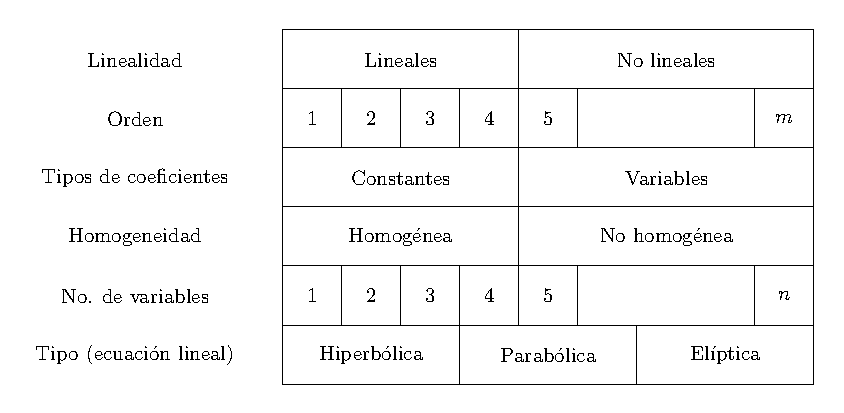
\includegraphics[scale=1.1]{Imagenes/Cuadro_Clasificacion_EDP.eps}
    \caption{Diagrama de clasificación de EDP.}
    \label{fig:figura_clasificacion_EDP}
\end{figure}
\end{enumerate}

%Ref. Zamora (2012) . Notas EDP 1.1.3 Problemas asociados.
\section{Problemas asociados.}

Se denomina un \emph{problema} a la EDP junto con un conjunto de condiciones dadas. Suponiendo una ecuación de la forma:
\begin{align}
F(x, t, u, u_{x}, u_{t}, u_{xx}, u_{xt}, u_{tt}) = 0
\label{eq:ecuacion_Z01_06}
\end{align}
es decir, una EDP de segundo orden en dos variables, se definen los distintos problemas.

\subsection{Problema de Cauchy.}
Este problema se conoce también como \emph{problema de valores iniciales}. Dado el carácter de segundo orden en las derivadas respecto al tiempo $t$ de la ec. (\ref{eq:ecuacion_Z01_06}, son necesarias dos condiciones sobre la solución $u(x, t)$. Estas son:
\begin{align}
u(x, 0) &= \phi (x) \label{eq:ecuacion_Z01_07} \\[0.5em]
u_{t}(x, 0) &= \psi (x) \label{eq:ecuacion_Z01_08}
\end{align}
donde $\phi$ y $\psi$ son funciones dadas en el intervalo de interés, y se ha elegido el tiempo inicial $t = 0$.
\par
Nótese que si en la EDP el orden mayor de la derivada respecto a $t$ fuese $N,$ entonces serían necesarias las derivadas parciales de $u$ respecto a $t$ desde el orden $0$ hasta el $N - 1$ evaluadas al tiempo $t = 0$ como condiciones.

\subsection{Problema de Dirichlet.}

Este es un tipo de problema conocido como de valores en la frontera. Dado el carácter de segundo orden en las derivadas respecto a la posición $x$ de la ec. (\ref{eq:ecuacion_Z01_06}), se necesitan dos condiciones sobre la solución $u(x, t)$. Suponiendo que se busca la solución para $a  \leq x \leq b$, $t \geq 0$, éstas son:
\begin{align}
u(a, t) &= f (t) \label{eq:ecuacion_Z01_09} \\[0.5em]
u(b, t) &= g(t) \label{eq:ecuacion_Z01_10}
\end{align}
donde $f$ y $g$ son funciones dadas, definidas para $t \geq 0$.
\par
Ahora notemos que si en la EDP el orden mayor de la derivada respecto a $x$ fuese $N$, entonces serían necesarios los valores de $u$ en $N$ distintos $x = a_{i}$ como condiciones. De manera general, el problema de Dirichlet \emph{prescribe} el valor de la función incógnita, $u$, en toda la \emph{frontera} de la región de interés.

\subsection{Problema de Neumann.}

Este es otro tipo de problema de \emph{valores en la frontera}. Suponiendo que se busca la solución para $a \leq x \leq b$, $t \geq 0$, las condiciones son en este caso las siguientes:
\begin{align}
u_{x}(a, t) &= f(t) \label{eq:ecuacion_Z01_11} \\[0.5em]
u_{x}(b, t) &= g(t) \label{eq:ecuacion_Z01_12}
\end{align}
donde $f$ y $g$ son funciones dadas, definidas para $t \geq 0$.
\par
Revisemos que si en la EDP el orden mayor de la derivada respecto a $x$ fuese $N$, entonces serían necesarios los valores de $u_{x}$ en $N$ distintos $x = a_{i}$ como condiciones. De manera general, el problema de Neumann \emph{prescribe} el valor de la derivada normal de la función incógnita, $\pdv*{u}{n}$, en toda la \emph{frontera} de la región de interés.

\subsection{Problema de Robin.}

Este problema \emph{de valores en la frontera} generaliza los dos anteriores. Suponiendo que se busca la solución para $a \leq x \leq b$, $t \geq 0$, las condiciones son:
\begin{align}
A_{1} \, u(a, t) + B_{1} \, u_{x}(a, t) &= f(t) \label{eq:ecuacion_Z01_13} \\[0.5em]
A_{2} \, u(b, t) + B_{2} \, u_{x}(b, t) &= g(t) \label{eq:ecuacion_Z01_14}
\end{align}
donde $f$ y $g$ son funciones dadas, definidas para $t \geq 0$, y $A_{1}, B_{1}, A_{2} y B_{2}$ son constantes dadas.
\par
Vale la pena remarcar que si en la EDP el orden mayor de la derivada respecto a $x$ fuese $N$, entonces serían necesarios los valores de $u$ y $u_{x}$ en $N$ distintos $x = a_{i}$ como condiciones. De manera general, el problema de Robin \emph{prescribe} el valor de una combinación lineal de la función incógnita $u$ y su derivada normal $\pdv*{u}{n}$ en toda la \emph{frontera} de la región de interés.

\subsection{Problemas Mixtos.}

Son problemas \emph{de valores en la frontera} y/o iniciales que mezclan condiciones de los anteriores. Suponiendo que se busca la solución para $a \leq x \leq b$, $t \geq 0$, un ejemplo sería el siguiente:
\begin{align}
A_{1} \, u(a, t) + B_{1} \, u(b, t) &= f(t) \label{eq:ecuacion_Z01_15} \\[0.5em]
A_{2} \, u_{x}(a, t) + B_{2} \, u_{x}(b, t) &= g(t) (\label{eq:ecuacion_Z01_16}
\end{align}
donde $f$ y $g$ son funciones dadas, definidas para $t \geq 0$, y $A_{1}, B_{1}, A_{2} y B_{2}$ son constantes dadas.
\par
Notemos que si en la EDP el orden mayor de la derivada respecto a $x$ fuese $N$, entonces serían necesarios los valores de $u$ o $u_{x}$ en $N$ distintos $x = a_{i}$ como condiciones. De manera general, los problemas mixtos \emph{prescriben} valores de combinaciones lineales de la función incógnita $u$ (o de su derivada normal $\pdv*{u}{n}$) evaluada en distintas partes de la \emph{frontera} de la región de interés.

\section{Problemas bien definidos.}

Se dice que un problema matemático que involucra EDP está \emph{bien definido} (o planteado) si satisface los siguientes requisitos:
\begin{enumerate}
\item Existencia: hay al menos una solución.
\item Unicidad: hay como máximo una solución.
\item Estabilidad: La solución depende continuamente de los datos.
\end{enumerate}

El primer requisito es una condición lógica obvia, pero debemos tener en cuenta que no podemos simplemente afirmar que el problema matemático tiene una solución solo porque el problema físico tiene una solución. Bien podemos estar desarrollando erróneamente un modelo matemático, digamos, que consiste en una EDP cuya solución puede no existir en absoluto. Lo mismo puede decirse del requisito de unicidad. Para reflejar realmente el problema físico que tiene una solución única, el problema matemático debe tener una solución única.
\par
Para problemas físicos, no es suficiente saber que el problema tiene una solución única. Por lo tanto, el último requisito no solo es útil sino también esencial. Para que la solución tenga importancia física, un pequeño cambio en los datos iniciales debe producir un pequeño cambio en la solución. Los datos de un problema físico se obtienen normalmente de experimentos y se aproximan para resolver el problema por métodos numéricos o aproximados. Es fundamental saber que el proceso de hacer una aproximación a los datos produce solo un pequeño cambio en la solución.

%Ref. http://www.scholarpedia.org/article/Partial_differential_equation
\section{Ecuaciones en la Física Matemática.}

\subsection{Ecuaciones lineales.}
Enumeremos algunas EDP conocidas:
\begin{enumerate}
    \item La ecuación de calor (ecuación parabólica)
\begin{align}
\text{\Large{$u_{t} - u_{xx} = 0$}}
\label{eq:ecuacion_S11}
\end{align}
donde las variables $t$ y $x$ juegan el papel de tiempo y una coordenada espacial, respectivamente. Revisemos que  en cuenta que la ecuación (\ref{eq:ecuacion_S11}) contiene solo un término con una derivada más alta.
\par
La ecuación (\ref{eq:ecuacion_S11}) se encuentra a menudo en la teoría de la transferencia de calor y de masa. Describe procesos térmicos inestables unidimensionales en medios inactivos o sólidos con difusividad térmica constante. Se utiliza una ecuación similar para estudiar los correspondientes procesos de intercambio de masa inestables unidimensionales con difusividad constante.
\item La ecuación de onda (ecuación hiperbólica)
\begin{align}
\text{\Large{$u_{tt} - u_{xx} = 0$}}
\label{eq:ecuacion_S12}
\end{align}
donde las variables $t$ y $x$ juegan el papel del tiempo y la coordenada espacial, respectivamente. Revisemos que los términos de la derivada más alta en la ecuación (\ref{eq:ecuacion_S12}) difieren en un signo.
\par
Esta ecuación también se conoce como \emph{ecuación de vibración de una cuerda}. A menudo se encuentra en elasticidad, aerodinámica, acústica y electrodinámica.
\item Ecuación de Laplace (ecuación elíptica)
\begin{align}
\text{\Large{$u_{xx} + u_{yy} = 0$}}
\label{eq:ecuacion_S14}
\end{align}
donde $x$ e $y$ juegan el papel de las coordenadas espaciales. Tomemos en cuenta que los términos de la derivada más alta en la ecuación (\ref{eq:ecuacion_S14}) tienen signos similares. La ecuación de Laplace a menudo se escribe brevemente como $\laplacian{u} = 0$, donde $\laplacian$ es el operador de Laplace o laplaciano.
\par
La ecuación de Laplace se encuentra a menudo en la teoría de transferencia de calor y masa, mecánica de fluidos, elasticidad, electrostática y otras áreas de la mecánica y la física. Por ejemplo, en la teoría de transferencia de calor y masa, esta ecuación describe la distribución de temperatura en estado estable en ausencia de fuentes de calor y sumideros en el dominio en estudio.
\end{enumerate}
\subsection{Ecuaciones no lineales.}
\begin{enumerate}
\item Ecuación no lineal de calor:
\begin{align}
\pdv{u}{t} = \pdv{x} \left[ f(u) \, \pdv{u}{x} \right]
\label{eq:ecuacion_S27}  
\end{align}
Esta ecuación describe procesos térmicos inestables unidimensionales en medios o sólidos en reposo en el caso en que la difusividad térmica depende de la temperatura, $f (u)> 0$. En el caso especial $f (w) \equiv 1$, la ecuación no lineal (\ref{eq:ecuacion_S27}) se convierte en la ecuación de calor lineal (\ref{eq:ecuacion_S11}).
\item Ecuación Kolmogorov-Petrovskii-Piskunov:
\begin{align}
\pdv{u}{t} = a \, \pdv[2]{w}{x} + f(u), \hspace{1cm} a > 0
\label{eq:ecuacion_S28}
\end{align}
Las ecuaciones de esta forma se encuentran a menudo en varios problemas de transferencia de masa y calor (siendo $f$ la reacción de cambio del volumen en una reacción química), teoría de la combustión, biología y ecología.
\par
En el caso especial de $f (u) \equiv 0$ y $a = 1$, la ecuación no lineal (\ref{eq:ecuacion_S28}) se convierte en la ecuación de calor lineal (\ref{eq:ecuacion_S11}).
\par
Observación: La ecuación (\ref{eq:ecuacion_S28}) también se le conoce como \emph{ecuación de calor con una fuente no lineal}.
\item Ecuación de Burgers:
\begin{align}
\pdv{w}{t} + u \, \pdv{u}{x} = \pdv[2]{u}{x}
\label{eq:ecuacion_S29}
\end{align}
Se ocupa para describir procesos ondulatorios en la dinámica de gases, hidrodinámica, en acústica y para el flujo del tráfico.
\item Ecuación de onda no lineal:
\begin{align}
\pdv[2]{u}{t} = \pdv{x} \left[ f(u) \, \pdv{u}{x} \right]
\label{eq:ecuacion_S30}
\end{align}
Esta ecuación se encuentra en dinámica de ondas y gases, con $f(u) > 0$. En el caso especial $f(u) \equiv 1$, la ecuación no lineal (\ref{eq:ecuacion_S30}) pasa a ser la ecuación de onda lineal (\ref{eq:ecuacion_S12}).
\item Ecuación Klein-Gordon no lineal:
\begin{align}
\pdv[2]{u}{t} = a \, \pdv[2]{u}{x} + f(u),\hspace{1cm} a > 0
\label{eq:ecuacion_S31}
\end{align}
Las ecuaciones de esta forma surgen en geometría diferencial y diversas áreas de la física: superconductividad, dislocaciones en cristales, ondas en materiales ferromagnéticos, pulsos de láser en medios bifásicos, entre otros. Para $f (u) \equiv 0$ y $a = 1$, la ecuación coincide con la ecuación de onda lineal.
\item Ecuación de Laplace no lineal:
\begin{align}
\pdv[2]{u}{x} + \pdv[2]{u}{y} = f(u)
\label{eq:ecuacion_S32}
\end{align}
A esta ecuación se le conoce también como \emph{ecuación estacionaria de calor con una fuente no lineal.}
\item Ecuación Monge-Ampere:
\begin{align}
\left( \pdv[2]{u}{x}{y} \right)^{2} - \pdv[2]{u}{x} \, \pdv[2]{u}{y} = (x, y)
\label{eq:ecuacion_S33}
\end{align}
Esta ecuación se encuentra en geometría diferencial, dinámica de gases y meteorología.
\end{enumerate}

\subsection{Ecuaciones lineales de derivadas de orden mayor.}

\begin{enumerate}
\item Ecuación de vibración de un varilla elástica:
\begin{align*}
\pdv[2]{w}{t} + a^{2} \, \pdv[4]{u}{x} = 0
\end{align*}
\item La ecuación biarmónica
\begin{align*}
\nabla^{4} = 0
\end{align*}
donde $\nabla^{4}$ es el operador biarmónico:
\begin{align*}
\nabla^{4} = \pdv[4]{x} + 2 \, \dfrac{\partial^{4}}{\partial x^{2} \, \partial y^{2}} + \pdv[4]{u}{y}
\end{align*}
La ecuación biarmónica se encuentra en problemas bidimensionales de elasticidad (como la función de tensión de Airy). También se utiliza para describir flujos lentos de fluidos viscosos incompresibles ($u$ es la función de corriente).
\end{enumerate}
Las ecuaciones que se han mencionado no son todas en la física matemática, habrá otras ecuaciones que extenderán este listado. Dependiendo del área de interés que decidas abordar, lo más seguro es que te encuentres con nuevas ecuaciones, que esperamos logres identificar las características principales, así como un abordaje para su solución. En el siguiente material de trabajo se revisará la técnica de solución: \emph{separación de variables.}

% \newpage

% \section{Ejercicio a cuenta.}

% \textbf{Ejercicio a cuenta (17).} Describe el tipo de ecuación y las regiones en las que es de tipo hiperbólica, parabólica y/o elíptica. Recuerda que debes de justificar el por qué de tu respuesta, es decir, deberás de realizar las operaciones y cálculos necesarios para tu respuesta.

% \begin{enumerate}[label=\alph*)]
% \item \Large{$u_{xx} - u_{xy} - 2 \, u_{yy} = 0$}
% \item \Large{$u_{xx} + 2 \, u_{xy} + u_{yy} = 0$}
% \item \Large{$2 \, u_{xx} + 4 \, u_{xy} + 3 \, u_{yy} - 5 \, u = 0$}
% \item \Large{$u_{xx} + 2 \, x \, u_{xy} + u_{yy} + (\cos x \, y) \, u_{x} - u = 0$}
% \item \Large{$y \, u_{xx} - 2 \, u_{xy} + e^{x} \, u_{yy} + u - 3 = 0$}
% \item \Large{$e^{x y} \, u_{xx} + (\sinh x) \, u_{yy} + u = 0$}
% \item \Large{$x \, u_{xx} + 2 \, x \, u_{xy} - y \, u_{yy} = 0$}
% \item \Large{$x \, u_{xx} + 2 \, x \, u_{xy} + y \, u_{yy} = 0$}
% \end{enumerate}
\end{document}